
\documentclass[12 pt, a4paper]{article}
\usepackage{mathptmx}
\usepackage{amsmath, latexsym}
\usepackage{amssymb}
\usepackage{enumerate}
\usepackage[utf8]{inputenc}
\usepackage{paralist}
\usepackage{enumitem}
\usepackage{lipsum}
%\pagenumbering{roman}
\usepackage{array}
\usepackage{textcmds}
\newcolumntype{P}[1]{>{\centering\arraybackslash}p{#1}}
\newcolumntype{M}[1]{>{\centering\arraybackslash}m{#1}}

\usepackage{longtable}
\usepackage{makecell}
\usepackage{changepage}


\usepackage{multirow}
\usepackage{multicol}
\usepackage[pdftex]{graphicx}
\usepackage[pdftex]{hyperref}
\usepackage{scalefnt}
\usepackage{setspace}
\usepackage{titlesec}
\usepackage{charter}
\newtheorem{proposition}{Proposition}
\usepackage{amsthm}
\usepackage{epsfig}
\usepackage{fancyhdr}
\usepackage{lastpage}
 
\usepackage{subfigure}
\usepackage{array,arydshln}
\usepackage{enumerate}
\usepackage{mathtools}
\usepackage{graphicx}
\usepackage{setspace}
\usepackage{color,soul}
\usepackage{enumitem}
\usepackage{tcolorbox}
\usepackage{tikz}
\usetikzlibrary{arrows}


%mkh
\usepackage{algorithm}
\usepackage{algorithmic}
\renewcommand{\algorithmicrequire}{\textbf{Inputs:}}
\renewcommand{\algorithmicensure}{\textbf{Outputs:}}

%%%%%%

\usepackage{amsmath}
\usetikzlibrary{decorations.markings}
\usepackage{verbatim}
\usetikzlibrary{positioning,fit,calc}
\tikzset{block/.style={draw,thick,text width=15cm,minimum height=1cm,align=center},
         line/.style={-latex}
}

\newtheorem{prop}{Proposition}
\newtheorem{thm}{Theorem}
\newtheorem{cor}[thm]{Corollary}
\newtheorem{lemma}[thm]{Lemma}
\mathchardef\mhyphen="2D % Define a "math hyphen"
\newtheorem{remark}{Remark}
\usepackage{array}
\newtheorem{theorem}{Theorem}
\theoremstyle{definition}
%\newtheorem{definition}{Definition}[section]
\newtheorem{definition}{Definition}
\usepackage{algorithm}
%\usepackage{algpseudocode}
\newenvironment{breakablealgorithm}
  {% \begin{breakablealgorithm}
   \begin{center}
     \refstepcounter{algorithm}% New algorithm
     \hrule height.8pt depth0pt \kern2pt% \@fs@pre for \@fs@ruled
     \renewcommand{\caption}[2][\relax]{% Make a new \caption
       {\raggedright\textbf{\ALG@name~\thealgorithm} ##2\par}%
       \ifx\relax##1\relax % #1 is \relax
         \addcontentsline{loa}{algorithm}{\protect\numberline{\thealgorithm}##2}%
       \else % #1 is not \relax
         \addcontentsline{loa}{algorithm}{\protect\numberline{\thealgorithm}##1}%
       \fi
       \kern2pt\hrule\kern2pt
     }
  }% \end{breakablealgorithm}
%\newtheorem{conjecture}{Conjecture}
%\usepackage{algpseudocode}
\makeatletter
\def\BState{\State\hskip-\ALG@thistlm}
\makeatother
\usepackage{titlesec}
\usepackage{float}
\tikzset{
    %Define standard arrow tip
    >=stealth',
    %Define style for boxes
    punkt/.style={
           rectangle,
           rounded corners,
           draw=black, very thick,
           text width=6.5em,
           minimum height=2em,
           text centered},
    % Define arrow style
    pil/.style={
           ->,
           thick,
           shorten <=3pt,
           shorten >=3pt,}
}

%\setcounter{secnumdepth}{4}
%\setcounter{page}{1}
\titleformat{\paragraph}
{\normalfont\normalsize\bfseries}{\theparagraph}{1em}{}
\titlespacing*{\paragraph}
{0pt}{3.25ex plus 1ex minus .2ex}{1.5ex plus .2ex}
\newcommand{\HRule}{\rule{\linewidth}{1mm}}
\topmargin = -30 mm
\textwidth = 175 mm
\textheight = 270 mm
\oddsidemargin = -10 mm
\evensidemargin = -10 mm

\setlist[description]{font=\itshape}
\usepackage[margin=.45in]{geometry}
%\pagenumbering{Arabic}
\usepackage{caption}
\captionsetup[figure]{font=small}

\begin{document}
   % \pagestyle{empty}
\vskip 0.2cm
    \begin{tabular}{rc}
        \multirow{0}{*}
        {
\includegraphics[scale=0.32]{logo.jpg}}                           & \hspace{1cm}\large\bf
            
        { IC 272: DATA SCIENCE - III} \\\
          \\ & \hspace{1cm}\large\bf{LAB ASSIGNMENT – I} \\ & \hspace{1cm}\bf{ Data visualization and statistics from data} 
          
            
          \end{tabular}
 \vskip 0.8cm

{\raggedleft{}\HRule}
  \\
  \textbf{Student's Name:} {name here} \hfill \textbf{Mobile No.:} {Mobile No. here} \\
  \noindent \textbf{Roll Number:} {Roll No. here} \hfill \textbf{Branch:}{ Branch here       } 
  
 \noindent\rule{18.7 cm}{2.3pt}



\section{}
\begin{table}[H]
	\caption{Mean, median, mode, minimum, maximum and standard deviation for all the attributes}
	\label{tab:Database}
	\centering
	\begin{tabular}{|c|c|c|c|c|c|c|c|}
	\hline
		\textbf{S. No.}& \textbf{Attribute} & \textbf{Mean} & \textbf{Median} & \textbf{Mode}&\textbf{Min.} &\textbf{Max.}&\textbf{S.D.} \\ \hline
		
		\textbf{1}          & pregs          &         &         &   & &&                \\ \hline
		\textbf{2}           & plas            &         &         &   &  &&               \\ \hline
		\textbf{3}          & pres (in mm Hg)          &         &         &   &        &&        \\ \hline
		\textbf{4}       & skin (in mm)         &         &         &   &           &&    \\ \hline
		\textbf{5}           & test (in mu U/mL)           &         &         &   &     &&          \\ \hline
			\textbf{6}           & BMI (in kg/m$^{2 }$)           &         &         &   &     &&          \\ \hline
		\textbf{7}          & pedi          &    &&     &         &   &                \\ \hline
		\textbf{8}       & Age (in years)          &   &&      &         &   &               \\ \hline
	
		
	\end{tabular}
	%\vspace{-4mm}
\end{table}

\textbf{\Large Inferences:}
\begin{enumerate}
   \item Infer if there is any relation between the magnitude of standard deviation and mean, mode and median values.(Hint : If standard deviation is close to zero; are mean, median and mode close to each other?)
   \item Inference 2(You may add or delete the number of inferences)
\end{enumerate}

\section{}
\textbf{a.}
\begin{figure}[H]
	\centering
	%\includegraphics[width=\linewidth,height=6cm]{ASLMK.jpg}
	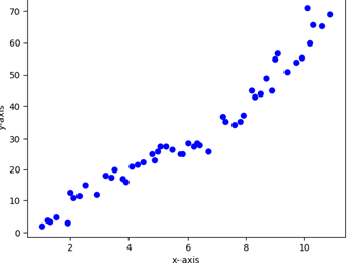
\includegraphics[width=8.5cm,height=6.65cm]{Scatter Plot.png}
	\caption{Scatter plot: Age (in years) vs. pregs}
	\label{Blockdia}
%	\vspace{-2mm}	
\end{figure}

\textbf{\Large Inferences:}
\begin{enumerate}
   \item Infer how the attribute 1 is correlated to attribute 2 based upon spread of the data points
   \item Inference based on density of points
   \item Inference 3(You may add or delete the number of inferences)
\\Note: The scatter plot above is for illustration purpose. Replace it with the scatter plot obtained by you. Rename x-axis legend and y-axis legends with appropriate attribute names with units.

\end{enumerate}

\begin{figure}[H]
	\centering
	%\includegraphics[width=\linewidth,height=6cm]{ASLMK.jpg}
	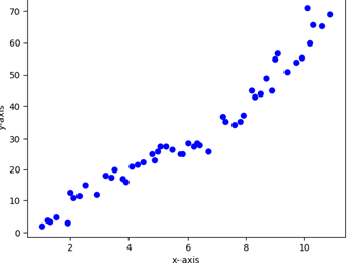
\includegraphics[width=8.5cm,height=6.65cm]{Scatter Plot.png}
	\caption{Scatter plot: Age (in years) vs. plas}
	\label{Blockdia}
%	\vspace{-2mm}	
\end{figure}

\textbf{\Large Inferences:}
\begin{enumerate}
   \item Infer how the attribute 1 is correlated to attribute 2 based upon spread of the data points
   \item Inference based on density of points
   \item Inference 3(You may add or delete the number of inferences)
\\Note: The scatter plot above is for illustration purpose. Replace it with the scatter plot obtained by you. Rename x-axis legend and y-axis legends with appropriate attribute names with units.

\end{enumerate}

\begin{figure}[H]
	\centering
	%\includegraphics[width=\linewidth,height=6cm]{ASLMK.jpg}
	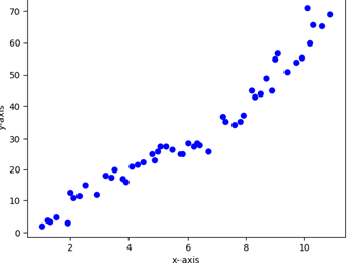
\includegraphics[width=8.5cm,height=6.65cm]{Scatter Plot.png}
	\caption{Scatter plot: Age (in years) vs. pres (in mm Hg)}
	\label{Blockdia}
%	\vspace{-2mm}	
\end{figure}

\textbf{\Large Inferences:}
\begin{enumerate}
   \item Infer how the attribute 1 is correlated to attribute 2 based upon spread of the data points
   \item Inference based on density of points
   \item Inference 3(You may add or delete the number of inferences)
\\Note: The scatter plot above is for illustration purpose. Replace it with the scatter plot obtained by you. Rename x-axis legend and y-axis legends with appropriate attribute names with units.

\end{enumerate}

\begin{figure}[H]
	\centering
	%\includegraphics[width=\linewidth,height=6cm]{ASLMK.jpg}
	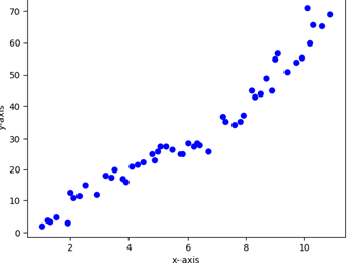
\includegraphics[width=8.5cm,height=6.65cm]{Scatter Plot.png}
	\caption{Scatter plot: Age (in years) vs. skin (in mm)}
	\label{Blockdia}
%	\vspace{-2mm}	
\end{figure}

\textbf{\Large Inferences:}
\begin{enumerate}
   \item Infer how the attribute 1 is correlated to attribute 2 based upon spread of the data points
   \item Inference based on density of points
   \item Inference 3(You may add or delete the number of inferences)\\Note: The scatter plot above is for illustration purpose. Replace it with the scatter plot obtained by you. Rename x-axis legend and y-axis legends with appropriate attribute names with units.

\end{enumerate}

\begin{figure}[H]
	\centering
	%\includegraphics[width=\linewidth,height=6cm]{ASLMK.jpg}
	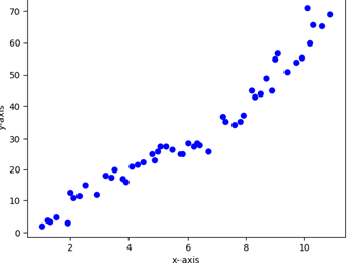
\includegraphics[width=8.5cm,height=6.65cm]{Scatter Plot.png}
	\caption{Scatter plot: Age (in years) vs. test (in mu U/mL)}
	\label{Blockdia}
%	\vspace{-2mm}	
\end{figure}

\textbf{\Large Inferences:}
\begin{enumerate}
   \item Infer how the attribute 1 is correlated to attribute 2 based upon spread of the data points
   \item Inference based on density of points
   \item Inference 3(You may add or delete the number of inferences)
\\Note: The scatter plot above is for illustration purpose. Replace it with the scatter plot obtained by you. Rename x-axis legend and y-axis legends with appropriate attribute names with units.

\end{enumerate}

\begin{figure}[H]
	\centering
	%\includegraphics[width=\linewidth,height=6cm]{ASLMK.jpg}
	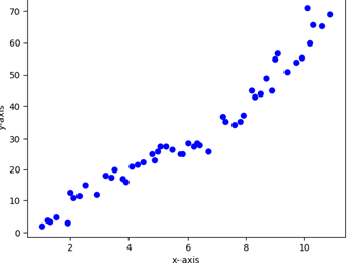
\includegraphics[width=8.5cm,height=6.65cm]{Scatter Plot.png}
	\caption{Scatter plot: Age (in years) vs. BMI (in kg/m$^{2 }$)}
	\label{Blockdia}
%	\vspace{-2mm}	
\end{figure}

\textbf{\Large Inferences:}
\begin{enumerate}
   \item Infer how the attribute 1 is correlated to attribute 2 based upon spread of the data points
   \item Inference based on density of points
   \item Inference 3(You may add or delete the number of inferences)
\\Note: The scatter plot above is for illustration purpose. Replace it with the scatter plot obtained by you. Rename x-axis legend and y-axis legends with appropriate attribute names with units.

\end{enumerate}

\begin{figure}[H]
	\centering
	%\includegraphics[width=\linewidth,height=6cm]{ASLMK.jpg}
	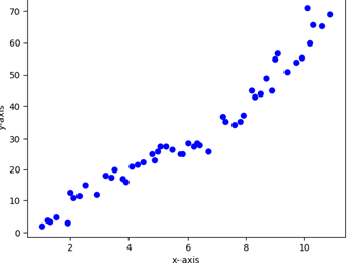
\includegraphics[width=8.5cm,height=6.65cm]{Scatter Plot.png}
	\caption{Scatter plot: Age (in years) vs. pedi}
	\label{Blockdia}
%	\vspace{-2mm}	
\end{figure}

\textbf{\Large Inferences:}
\begin{enumerate}
   \item Infer how the attribute 1 is correlated to attribute 2 based upon spread of the data points
   \item Inference based on density of points
   \item Inference 3(You may add or delete the number of inferences)
\\Note: The scatter plot above is for illustration purpose. Replace it with the scatter plot obtained by you. Rename x-axis legend and y-axis legends with appropriate attribute names with units.

\end{enumerate}



\noindent\textbf{b.}
\begin{figure}[H]
	\centering
	%\includegraphics[width=\linewidth,height=6cm]{ASLMK.jpg}
	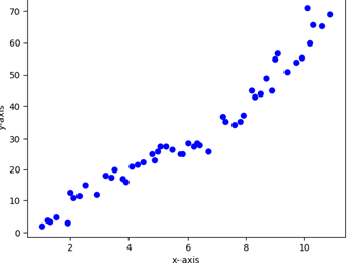
\includegraphics[width=8.5cm,height=6.65cm]{Scatter Plot.png}
	\caption{Scatter plot: BMI (in kg/m$^{2 }$) vs. pregs}
	\label{Blockdia}
%	\vspace{-2mm}	
\end{figure}

\textbf{\Large Inferences:}
\begin{enumerate}
   \item Infer how the attribute 1 is correlated to attribute 2 based upon spread of the data points
   \item Inference based on density of points
   \item Inference 3(You may add or delete the number of inferences)
\\Note: The scatter plot above is for illustration purpose. Replace it with the scatter plot obtained by you. Rename x-axis legend and y-axis legends with appropriate attribute names with units.

\end{enumerate}

\begin{figure}[H]
	\centering
	%\includegraphics[width=\linewidth,height=6cm]{ASLMK.jpg}
	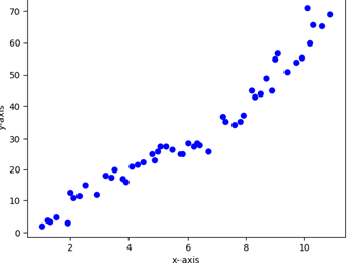
\includegraphics[width=8.5cm,height=6.65cm]{Scatter Plot.png}
	\caption{Scatter plot: BMI (in kg/m$^{2 }$) vs. plas}
	\label{Blockdia}
%	\vspace{-2mm}	
\end{figure}

\textbf{\Large Inferences:}
\begin{enumerate}
   \item Infer how the attribute 1 is correlated to attribute 2 based upon spread of the data points
   \item Inference based on density of points
   \item Inference 3(You may add or delete the number of inferences)
\\Note: The scatter plot above is for illustration purpose. Replace it with the scatter plot obtained by you. Rename x-axis legend and y-axis legends with appropriate attribute names with units.

\end{enumerate}

\begin{figure}[H]
	\centering
	%\includegraphics[width=\linewidth,height=6cm]{ASLMK.jpg}
	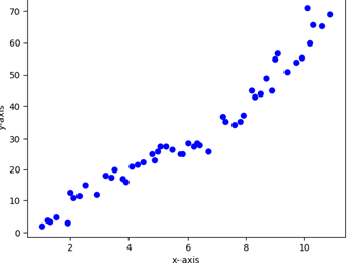
\includegraphics[width=8.5cm,height=6.65cm]{Scatter Plot.png}
	\caption{Scatter plot: BMI (in kg/m$^{2 }$) vs. pres (in mm Hg)}
	\label{Blockdia}
%	\vspace{-2mm}	
\end{figure}

\textbf{\Large Inferences:}
\begin{enumerate}
   \item Infer how the attribute 1 is correlated to attribute 2 based upon spread of the data points
   \item Inference based on density of points
   \item Inference 3(You may add or delete the number of inferences)
\\Note: The scatter plot above is for illustration purpose. Replace it with the scatter plot obtained by you. Rename x-axis legend and y-axis legends with appropriate attribute names with units.

\end{enumerate}

\begin{figure}[H]
	\centering
	%\includegraphics[width=\linewidth,height=6cm]{ASLMK.jpg}
	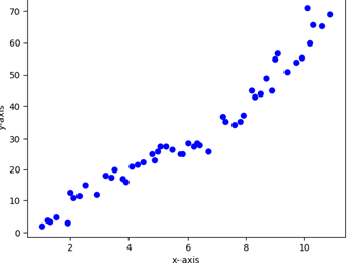
\includegraphics[width=8.5cm,height=6.65cm]{Scatter Plot.png}
	\caption{Scatter plot: BMI (in kg/m$^{2 }$) vs. skin (in mm)}
	\label{Blockdia}
%	\vspace{-2mm}	
\end{figure}

\textbf{\Large Inferences:}
\begin{enumerate}
   \item Infer how the attribute 1 is correlated to attribute 2 based upon spread of the data points
   \item Inference based on density of points
   \item Inference 3(You may add or delete the number of inferences)
\\Note: The scatter plot above is for illustration purpose. Replace it with the scatter plot obtained by you. Rename x-axis legend and y-axis legends with appropriate attribute names with units.

\end{enumerate}

\begin{figure}[H]
	\centering
	%\includegraphics[width=\linewidth,height=6cm]{ASLMK.jpg}
	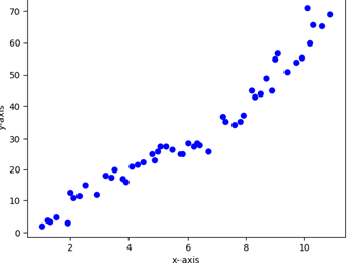
\includegraphics[width=8.5cm,height=6.65cm]{Scatter Plot.png}
	\caption{Scatter plot: BMI (in kg/m$^{2 }$) vs. test (in mu U/mL)}
	\label{Blockdia}
%	\vspace{-2mm}	
\end{figure}

\textbf{\Large Inferences:}
\begin{enumerate}
   \item Infer how the attribute 1 is correlated to attribute 2 based upon spread of the data points
   \item Inference based on density of points
   \item Inference 3(You may add or delete the number of inferences)
\\Note: The scatter plot above is for illustration purpose. Replace it with the scatter plot obtained by you. Rename x-axis legend and y-axis legends with appropriate attribute names with units.

\end{enumerate}



\begin{figure}[H]
	\centering
	%\includegraphics[width=\linewidth,height=6cm]{ASLMK.jpg}
	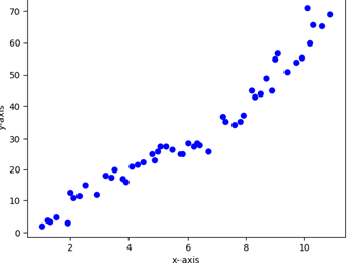
\includegraphics[width=8.5cm,height=6.65cm]{Scatter Plot.png}
	\caption{Scatter plot: BMI (in kg/m$^{2 }$) vs. pedi}
	\label{Blockdia}
%	\vspace{-2mm}	
\end{figure}

\textbf{\Large Inferences:}
\begin{enumerate}
   \item Infer how the attribute 1 is correlated to attribute 2 based upon spread of the data points
   \item Inference based on density of points
   \item Inference 3(You may add or delete the number of inferences)
\\Note: The scatter plot above is for illustration purpose. Replace it with the scatter plot obtained by you. Rename x-axis legend and y-axis legends with appropriate attribute names with units.

\end{enumerate}

\begin{figure}[H]
	\centering
	%\includegraphics[width=\linewidth,height=6cm]{ASLMK.jpg}
	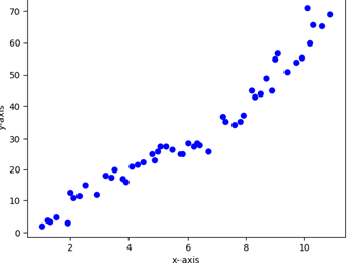
\includegraphics[width=8.5cm,height=6.65cm]{Scatter Plot.png}
	\caption{Scatter plot: BMI (in kg/m$^{2 }$) vs. Age (in years)}
	\label{Blockdia}
%	\vspace{-2mm}	
\end{figure}

\textbf{\Large Inferences:}
\begin{enumerate}
   \item Infer how the attribute 1 is correlated to attribute 2 based upon spread of the data points
   \item Inference based on density of points
   \item Inference 3(You may add or delete the number of inferences)
\\Note: The scatter plot above is for illustration purpose. Replace it with the scatter plot obtained by you. Rename x-axis legend and y-axis legends with appropriate attribute names with units.

\end{enumerate}


\section{} 
\textbf{a.}
\begin{table}[H]
	\caption{Correlation coefficient value computed between age and all other attributes}
	\label{tab:Database}
	\centering
	\begin{tabular}{|c|c|c|}
	\hline
		\textbf{S. No.}& \textbf{Attribute} & \textbf{Correlation coefficient value}  \\ \hline
		
		\textbf{1}          & pregs          &                    \\ \hline
		\textbf{2}           & plas            &        \\ \hline
		\textbf{3}          & pres (in mm Hg)          &            \\ \hline
		\textbf{4}       & skin (mm)         &         \\ \hline
		\textbf{5}           & test (in mu U/mL)           &        \\ \hline
			\textbf{6}           & BMI (in kg/m$^{2 }$)           &               \\ \hline
		\textbf{7}          & pedi          &     \\ \hline
		\textbf{8}       & Age (in years)          &            \\ \hline
	
		
	\end{tabular}
	%\vspace{-4mm}
\end{table}

\textbf{\Large Inferences:}
\begin{enumerate}
   \item From the magnitude of correlation coefficient value, comment on the degree of correlation between age and each of the attribute.
    \item From the sign of correlation coefficient value, comment whether with increase or decrease in age each of the attributes will increase or decrease.
    \item Relate and comment on the value of correlation coefficient with corresponding scatter plots.
   \item Inference 4(You may add or delete the number of inferences)
\end{enumerate}

\clearpage
\textbf{b.}
\begin{table}[H]
	\caption{Correlation coefficient value computed between BMI and all other attributes}
	\label{tab:Database}
	\centering
	\begin{tabular}{|c|c|c|}
	\hline
		\textbf{S. No.}& \textbf{Attribute} & \textbf{Correlation coefficient value}  \\ \hline
		
		\textbf{1}          & pregs          &                    \\ \hline
		\textbf{2}           & plas            &        \\ \hline
		\textbf{3}          & pres (in mm Hg)          &            \\ \hline
		\textbf{4}       & skin (mm)         &         \\ \hline
		\textbf{5}           & test (in mu U/mL)           &        \\ \hline
			\textbf{6}           & BMI (in kg/m$^{2 }$)           &               \\ \hline
		\textbf{7}          & pedi          &     \\ \hline
		\textbf{8}       & Age (in years)          &            \\ \hline
	
		
	\end{tabular}
	%\vspace{-4mm}
\end{table}

\textbf{\Large Inferences:}
\begin{enumerate}
   \item From the magnitude of correlation coefficient value, comment on the degree of correlation between BMI and each of the attribute.
    \item From the sign of correlation coefficient value, comment whether with increase or decrease in BMI each of the attributes will increase or decrease.
        \item Relate and comment on the value of correlation coefficient with corresponding scatter plots.
   \item Inference 4(You may add or delete the number of inferences)
\end{enumerate}

\section{}
\textbf{a.}
\begin{figure}[H]
	\centering
	%\includegraphics[width=\linewidth,height=6cm]{ASLMK.jpg}
	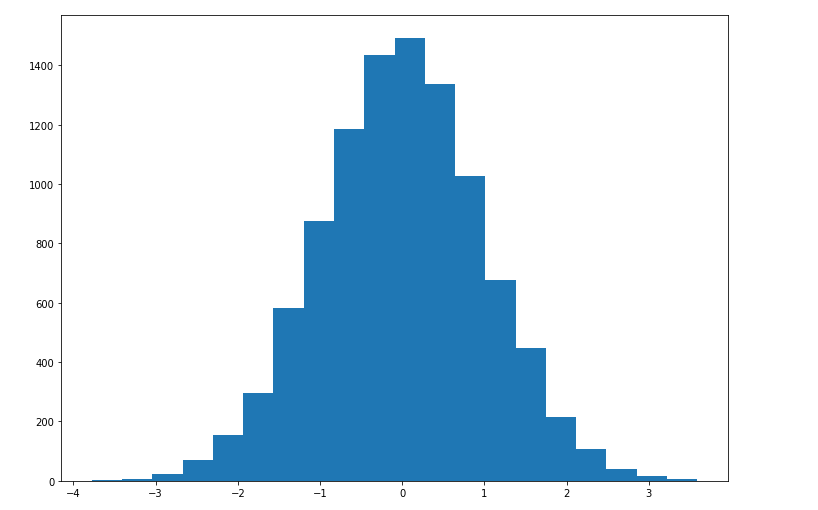
\includegraphics[width=11.5cm,height=6.65cm]{histogram.png}
	\caption{Histogram depiction of attribute pregs}
	\label{Blockdia}
%	\vspace{-2mm}	
\end{figure}

\textbf{\Large Inferences:}
\begin{enumerate}

   \item Infer the frequency of each bin referring to its height.
   \item From the histogram, infer in which of the bins mode of the attribute pregs lies.
   \item Inference 3(You may add or delete the number of inferences)
\\Note: The histogram plot above is for illustration purpose. Replace it with the histogram plot obtained by you. Rename x-axis legend and y-axis legends with appropriate attribute names with units.

\end{enumerate}
\textbf{b.}
\begin{figure}[H]
	\centering
	%\includegraphics[width=\linewidth,height=6cm]{ASLMK.jpg}
	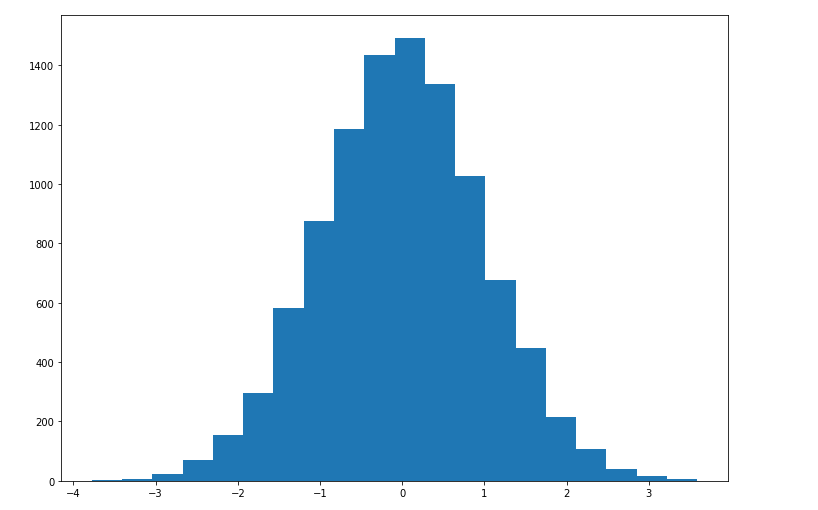
\includegraphics[width=11.5cm,height=6.65cm]{histogram.png}
	\caption{Histogram depiction of attribute skin}
	\label{Blockdia}
%	\vspace{-2mm}	
\end{figure}

\textbf{\Large Inferences:}
\begin{enumerate}
      \item Infer the frequency of each bin referring to its height.
   \item From the histogram, infer in which of the bins mode of the attribute skin lies.

   \item Inference 3(You may add or delete the number of inferences)
\\Note: The histogram plot above is for illustration purpose. Replace it with the histogram plot obtained by you. Rename x-axis legend and y-axis legends with appropriate attribute names with units.

\end{enumerate}

\section{}
\begin{figure}[H]
	\centering
	%\includegraphics[width=\linewidth,height=6cm]{ASLMK.jpg}
	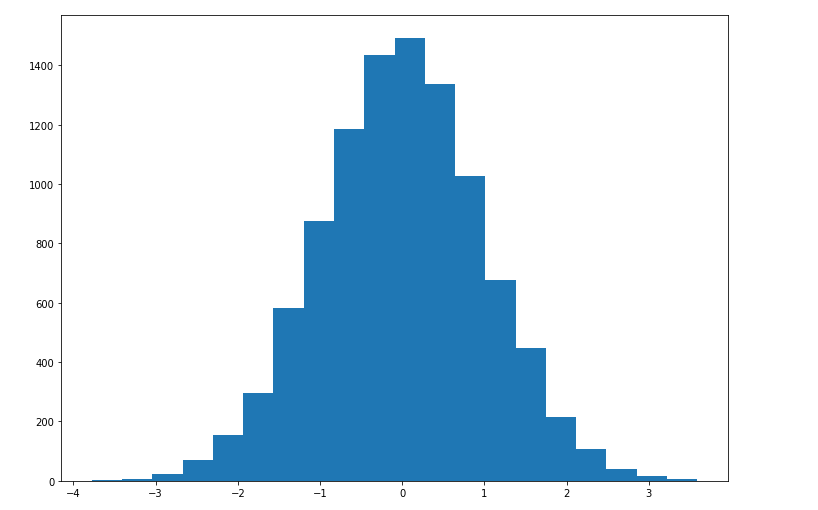
\includegraphics[width=11.5cm,height=6.65cm]{histogram.png}
	\caption{Histogram depiction of attribute pregs for class 0}
	\label{Blockdia}
%	\vspace{-2mm}	
\end{figure}

\begin{figure}[H]
	\centering
	%\includegraphics[width=\linewidth,height=6cm]{ASLMK.jpg}
	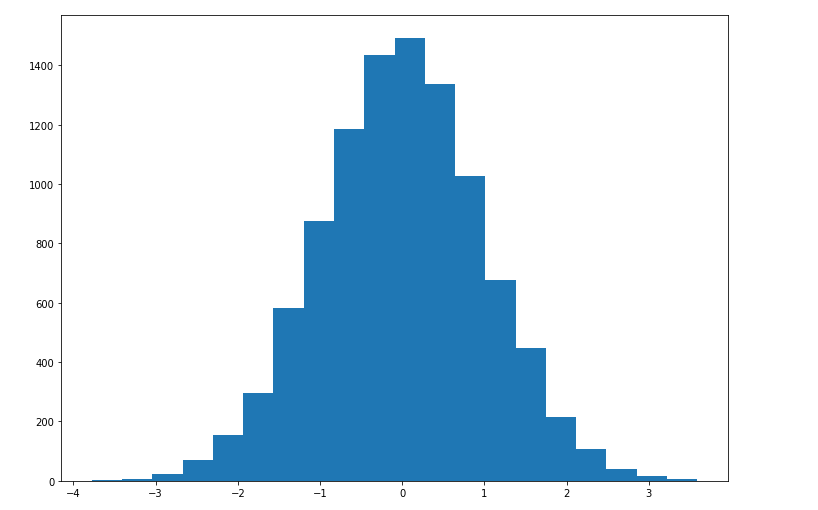
\includegraphics[width=11.5cm,height=6.65cm]{histogram.png}
	\caption{Histogram depiction of attribute pregs for class 1}
	\label{Blockdia}
%	\vspace{-2mm}	
\end{figure}

\textbf{\Large Inferences:}
\begin{enumerate}
   \item From the histogram, infer in which of the bins mode of the attribute pregs lies for class 0 and 1.
   \item Compare and contrast the frequency referring to the height of each bin for class 0 and 1
   \item Inference 3(You may add or delete the number of inferences)
\\Note: The histogram plot above is for illustration purpose. Replace it with the histogram plot obtained by you. Rename x-axis legend and y-axis legends with appropriate attribute names with units.

\end{enumerate}

\section{}

\begin{figure}[H]
	\centering
	%\includegraphics[width=\linewidth,height=6cm]{ASLMK.jpg}
	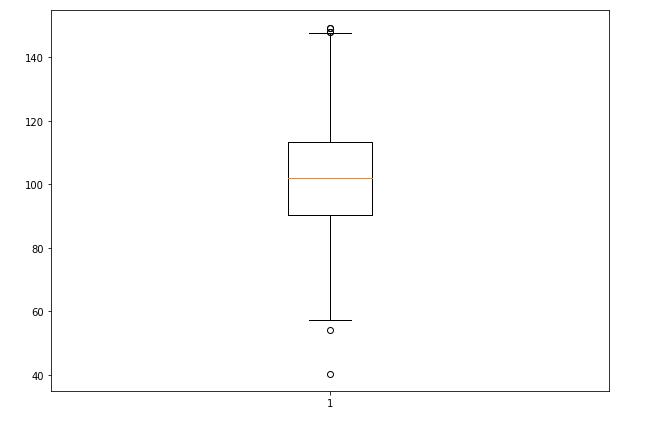
\includegraphics[width=8.5cm,height=6.65cm]{boxplot.png}
	\caption{Boxplot for attribute pregs}
	\label{Blockdia}
%	\vspace{-2mm}	
\end{figure}

\textbf{\Large Inferences:}
\begin{enumerate}
   \item Inference on outliers and their values.
   \item Infer the Inter quartile range.
   \item Infer the variability of attribute.
   \item Infer the skewness of the data.
 \item Relate with the values observed in Q1. \item Inference 6 (You may add or delete the number of inferences)
\\Note: The boxplot above is for illustration purpose. Replace it with the boxplot obtained by you. Rename x-axis legend and y-axis legends with appropriate attribute names with units.

\end{enumerate}

\begin{figure}[H]
	\centering
	%\includegraphics[width=\linewidth,height=6cm]{ASLMK.jpg}
	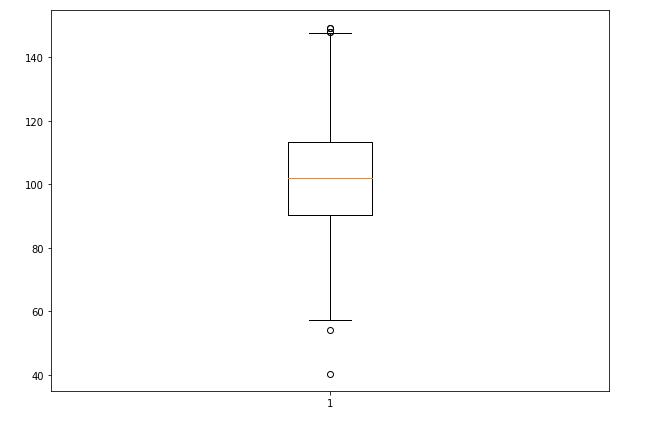
\includegraphics[width=8.5cm,height=6.65cm]{boxplot.png}
	\caption{Boxplot for attribute plas}
	\label{Blockdia}
%	\vspace{-2mm}	
\end{figure}

\textbf{\Large Inferences:}
\begin{enumerate}
   \item Inference on outliers and their values.
   \item Infer the Inter quartile range.
   \item Infer the variability of attribute.
   \item Infer the skewness of the data.
 \item Relate with the values observed in Q1. \item Inference 6 (You may add or delete the number of inferences)
\\Note: The boxplot above is for illustration purpose. Replace it with the boxplot obtained by you. Rename x-axis legend and y-axis legends with appropriate attribute names with units.

\end{enumerate}

\begin{figure}[H]
	\centering
	%\includegraphics[width=\linewidth,height=6cm]{ASLMK.jpg}
	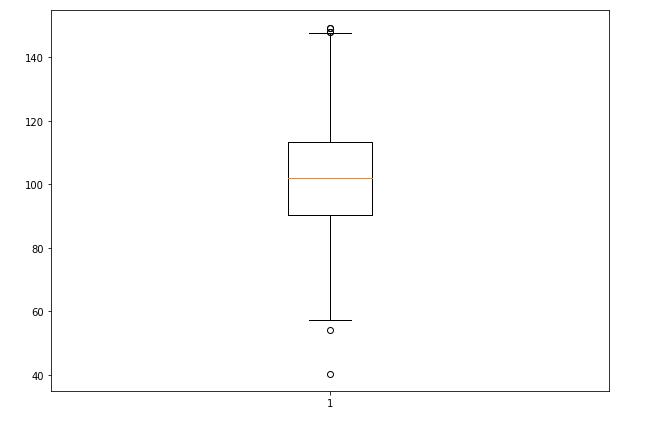
\includegraphics[width=8.5cm,height=6.65cm]{boxplot.png}
	\caption{Boxplot for attribute pres (in mm Hg)}
	\label{Blockdia}
%	\vspace{-2mm}	
\end{figure}

\textbf{\Large Inferences:}
\begin{enumerate}
   \item Inference on outliers and their values.
   \item Infer the Inter quartile range.
   \item Infer the variability of attribute.
   \item Infer the skewness of the data.
 \item Relate with the values observed in Q1. \item Inference 6 (You may add or delete the number of inferences)
\\Note: The boxplot above is for illustration purpose. Replace it with the boxplot obtained by you. Rename x-axis legend and y-axis legends with appropriate attribute names with units.

\end{enumerate}

\begin{figure}[H]
	\centering
	%\includegraphics[width=\linewidth,height=6cm]{ASLMK.jpg}
	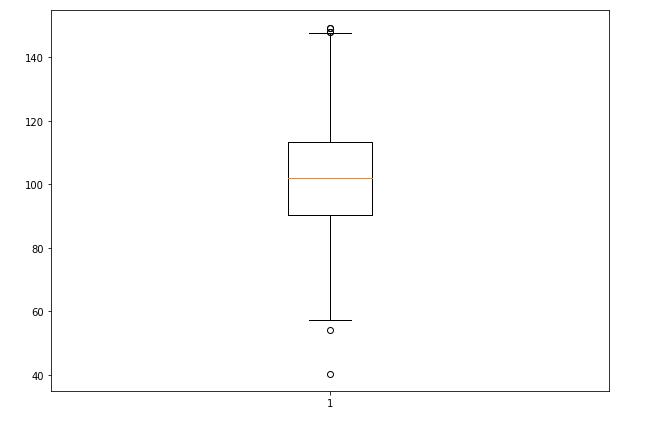
\includegraphics[width=8.5cm,height=6.65cm]{boxplot.png}
	\caption{Boxplot for attribute skin (in mm)}
	\label{Blockdia}
%	\vspace{-2mm}	
\end{figure}

\textbf{\Large Inferences:}
\begin{enumerate}
   \item Inference on outliers and their values.
   \item Infer the Inter quartile range.
   \item Infer the variability of attribute.
   \item Infer the skewness of the data.
 \item Relate with the values observed in Q1. \item Inference 6 (You may add or delete the number of inferences)
\\Note: The boxplot above is for illustration purpose. Replace it with the boxplot obtained by you. Rename x-axis legend and y-axis legends with appropriate attribute names with units.

\end{enumerate}

\begin{figure}[H]
	\centering
	%\includegraphics[width=\linewidth,height=6cm]{ASLMK.jpg}
	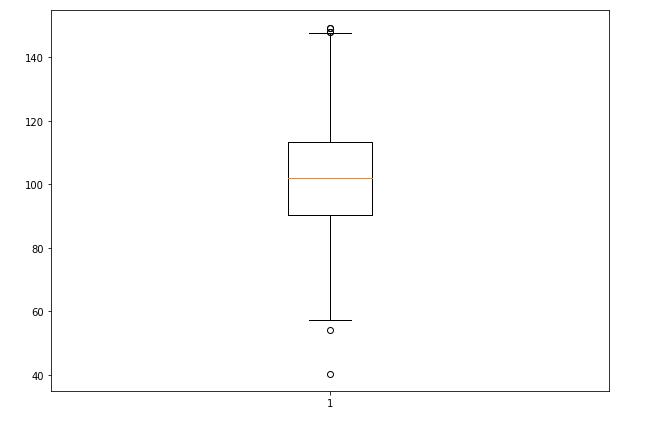
\includegraphics[width=8.5cm,height=6.65cm]{boxplot.png}
	\caption{Boxplot for attribute test (in mu U/mL)}
	\label{Blockdia}
%	\vspace{-2mm}	
\end{figure}

\textbf{\Large Inferences:}
\begin{enumerate}
   \item Inference on outliers and their values.
   \item Infer the Inter quartile range.
   \item Infer the variability of attribute.
   \item Infer the skewness of the data.
 \item Relate with the values observed in Q1. \item Inference 6 (You may add or delete the number of inferences)
\\Note: The boxplot above is for illustration purpose. Replace it with the boxplot obtained by you. Rename x-axis legend and y-axis legends with appropriate attribute names with units.

\end{enumerate}

\begin{figure}[H]
	\centering
	%\includegraphics[width=\linewidth,height=6cm]{ASLMK.jpg}
	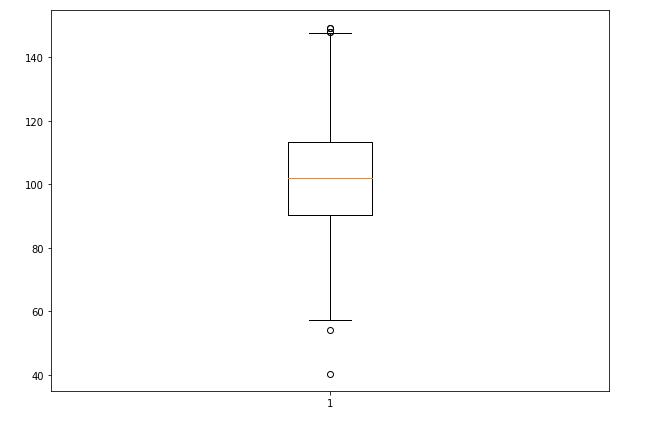
\includegraphics[width=8.5cm,height=6.65cm]{boxplot.png}
	\caption{Boxplot for attribute BMI(kg/m$^{2}$)}
	\label{Blockdia}
%	\vspace{-2mm}	
\end{figure}

\textbf{\Large Inferences:}
\begin{enumerate}
   \item Inference on outliers and their values.
   \item Infer the Inter quartile range.
   \item Infer the variability of attribute.
   \item Infer the skewness of the data.
 \item Relate with the values observed in Q1. \item Inference 6 (You may add or delete the number of inferences)
\\Note: The boxplot above is for illustration purpose. Replace it with the boxplot obtained by you. Rename x-axis legend and y-axis legends with appropriate attribute names with units.

\end{enumerate}

\begin{figure}[H]
	\centering
	%\includegraphics[width=\linewidth,height=6cm]{ASLMK.jpg}
	\includegraphics[width=8.5cm,height=6.65cm]{boxplot.png}
	\caption{Boxplot for attribute pedi}
	\label{Blockdia}
%	\vspace{-2mm}	
\end{figure}

\textbf{\Large Inferences:}
\begin{enumerate}
   \item Inference on outliers and their values.
   \item Infer the Inter quartile range.
   \item Infer the variability of attribute.
   \item Infer the skewness of the data.
 \item Relate with the values observed in Q1. \item Inference 6 (You may add or delete the number of inferences)
\\Note: The boxplot above is for illustration purpose. Replace it with the boxplot obtained by you. Rename x-axis legend and y-axis legends with appropriate attribute names with units.

\end{enumerate}

\begin{figure}[H]
	\centering
	%\includegraphics[width=\linewidth,height=6cm]{ASLMK.jpg}
	\includegraphics[width=8.5cm,height=6.65cm]{boxplot.png}
	\caption{Boxplot for attribute Age (in years)}
	\label{Blockdia}
%	\vspace{-2mm}	
\end{figure}

\textbf{\Large Inferences:}
\begin{enumerate}
   \item Inference on outliers and their values.
   \item Infer the Inter quartile range.
   \item Infer the variability of attribute.
   \item Infer the skewness of the data.
 \item Relate with the values observed in Q1. \item Inference 6 (You may add or delete the number of inferences)
\\Note: The boxplot above is for illustration purpose. Replace it with the boxplot obtained by you. Rename x-axis legend and y-axis legends with appropriate attribute names with units.

\end{enumerate}
%delete this begin
~\\~\\~\\~\\
\bf{\large{{Guidelines for Report (Delete this while you submit the report):\\}}}
\\
~

  \begin{itemize}
  
     \item The plot/graph/figure/table should be centre justified with sequence number and caption.
     \item Inferences should be written as a numbered list.
     \item Use specific and technical terms to write inferences
     \item Values observed/calculated should be rounded off to three decimal places.
     \item The quantities which have units should be written with units.
   \end{itemize}

%dete this end here
\end{document}
